\begin{frame}{Solution}{Context Engine}
\begin{block}{Context}
Information that characterizes the situation of a participant in an interaction.
\end{block}
\end{frame}

\begin{frame}{Solution}{Context Engine}
\begin{figure}[h]
\centering
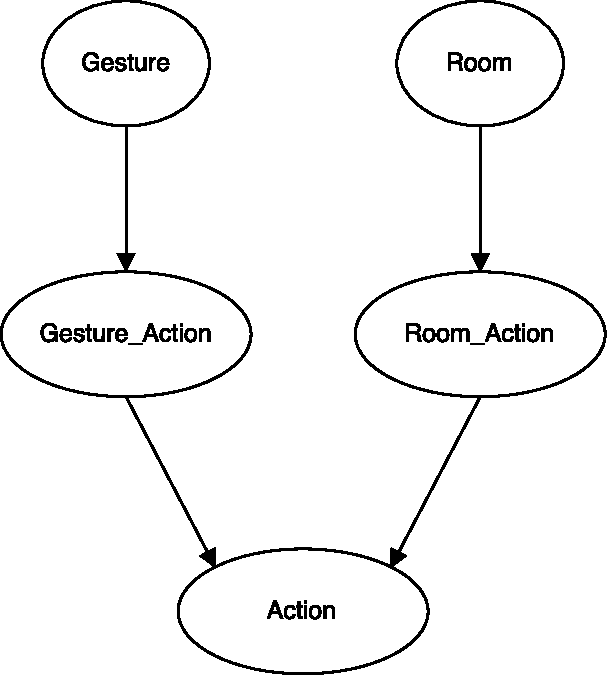
\includegraphics[width=0.4\textwidth]{../images/bayesian-network-simple}
\caption{Bayesian network used in the implementation.}
\end{figure}
\end{frame}

\begin{frame}{Solution}{Context Engine}
\begin{textblock*}{1.5cm}(0.5cm,2.4cm)
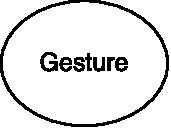
\includegraphics[width=1.5cm]{../images/bayesian-network-gesture-node}
\end{textblock*}
\begin{itemize}
\item Gesture recognition on the wearable, producing \emph{gesture traces}.
\item Distance between the gesture trace and \emph{gesture templates}.
\item Translation of distances to beliefs in the \emph{Gesture\_Action\_Node}. 
\end{itemize}
\end{frame}

\begin{frame}{Solution}{Context Engine}
\begin{textblock*}{1.5cm}(0.5cm,2.4cm)
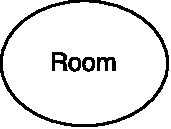
\includegraphics[width=1.5cm]{../images/bayesian-network-room-node}
\end{textblock*}
\begin{itemize}
\item Positioning of the wearable using BLE beacons, focusing on the one we measure the highest RSSI from.
\item Counting references to rooms we discover beacons in.
\end{itemize}
\end{frame}

%%% Local Variables:
%%% mode: latex
%%% TeX-master: "../AAUsimpletheme"
%%% End:
